\todo{Wichtige Begriffe erklären}
\subsection{Flüchtige Speicher}
	Bei flüchtigem Speicher handelt es sich um Speicher, die ihre Information ohne Spannungsversorgung verlieren.
	Das Random-Access-Memory(RAM) steht für den wahlfreien Zugriff, also dass jede Speicherzelle über die Speicheradresse direkt angesprochen werden kann. Man unterscheidet zwischen zwei Arten:
	\subsubsection{SRAM}
		Beim SRAM wird die Ladung in einem Flip-Flog (2 CMOS Inverter) gespeichert. Diese werden mit 6 Transistorzellen realisiert. 
		\newline
		% Bild SRAM Zelle
		\begin{center}
			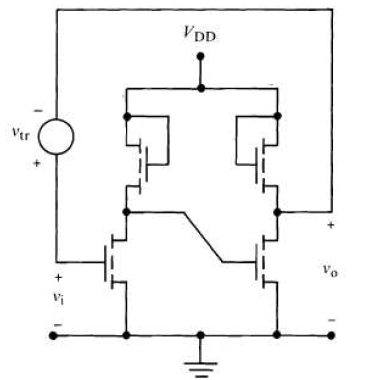
\includegraphics[width=0.3\linewidth]{Kapitel/Kap07/SRAMZelle.png}
		\end{center}		
		Vorteil: sehr schnell, behält Information auch ohne Taktspannung, kein Refresh nötig
		\newline
		Nachteil: geringere Speicherdichte
		\newline
		Mit Hilfe einer Pufferbatterie kann der SRAM zu einem nichtflüchtigen Speicher gewandelt werden.
	\subsubsection{DRAM}
		Die Informationen werden in Form des Ladezustandes eines  MOS-Kondensator gespeichert. Die Realisierung benötigt daher nur 1 Transistorzelle und einen Kondensator.
		\begin{center}
			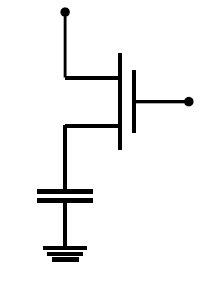
\includegraphics[width=0.2\linewidth]{Kapitel/Kap07/DRAMZelle.png}
		\end{center}
		Der Kondensator entlädt sich bei den kleinen möglichen Kapazitäten durch die auftretenden Leckströme schnell. Ein Refresh mit Taktspannung etwa alle 32 ms ist notwendig. Das Lesen ist destruktiv. Auch hier ist ein Refresh notwendig.
		\newline
		Vorteil: wenig Platzbedarf, gute Skalierbarkeit, kostengünstig
		\newline
		Nachteil: Refresh nötig
		\newline
		
		\textbf{Technische Realisierung}
		\newline
		Die technische Realisierung des Kondensatoren wurde in der Vergangenheit auf der Oberfläche des Halbleiters realisiert und war damit sehr platzintensiv. 
		\begin{center}
			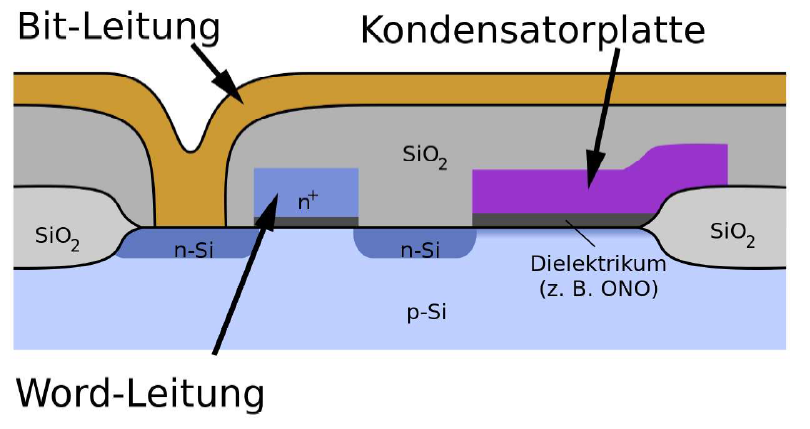
\includegraphics[width=0.3\linewidth]{Kapitel/Kap07/Condensatorimplmentierung_Alt}
		\end{center}
		
		Heutzutage findet die Implementierung entweder in Form eines Grabens (Trench) statt, wobei der Kondensator durch Ätzen eines 5-10 $\mu m$ tiefen Loches im Substrat erzeugt wird. 
		\newline
		Alternativ gibt es die Stacked Form, wobei der Kondensator über dem Transistor aufgebaut (gestapelt) wird.
		
		\begin{center}
			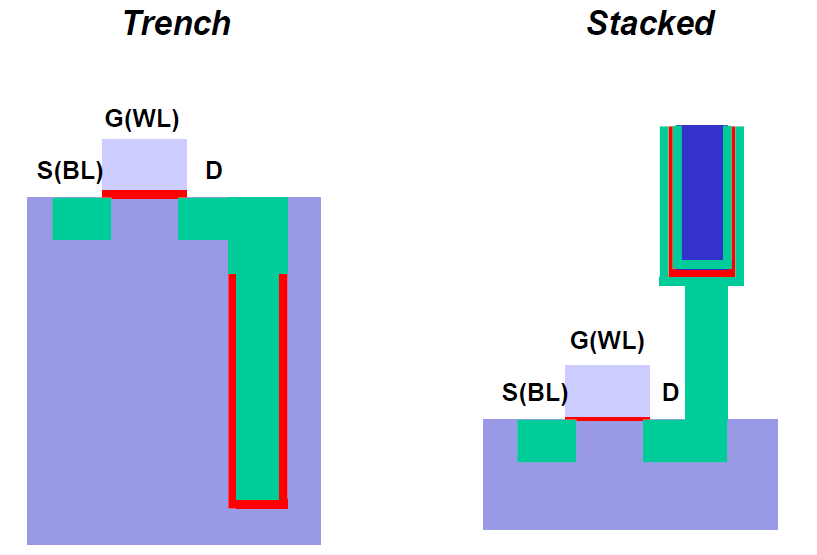
\includegraphics[width=0.4\linewidth]{Kapitel/Kap07/TrenchAndStack}
		\end{center}
		

\subsection{Nichtflüchtige Speicher}
	Nichtflüchtiger Speicher bewahren gespeicherte Information auch ohne Spannungsversorgung.
	Auch hier gibt es verschiedene Formen:
	\subsubsection{ROM}
		\begin{itemize}
			\item Datenspeicher, der nur lesbar ist, im normalen Betrieb aber nicht beschrieben werden kann.
			\item Information meist bei der Chip-Produktion vom Hersteller eingeschrieben
		\end{itemize}
	\subsubsection{PROM}
		\begin{itemize}
			\item einmalige Programmierung durch Anwender
			\item Schreiben destruktiv und nicht reversibel (z.B. Durchbrennen spezieller Leitbahnen)
			\item Programmierung durch Ausbrennwiderständen oder kurzgeschlossene Sperrschicht
		\end{itemize}
	\subsubsection{EPROM}
		\begin{itemize}
			\item beschränktes Löschen und Programmieren
			\item langsames Schreiben erfolgt elektrisch
			\item  Löschen (meist komplett) erfolgt z.B. mit UV-Licht
		\end{itemize}
	\subsubsection{EEPROM}
		\begin{itemize}
			\item einzelne Speicherzellen können elektrisch gelöscht und wieder programmiert werden		
			\item zusätzliche Auswahltransistoren für die Zellen
			\item Die Be- und Endladung erfolgt i.d.R. über ein Floating Gate (bewirkt Verschiebung der Schwellspannung am Steuergate)
			\begin{center}
				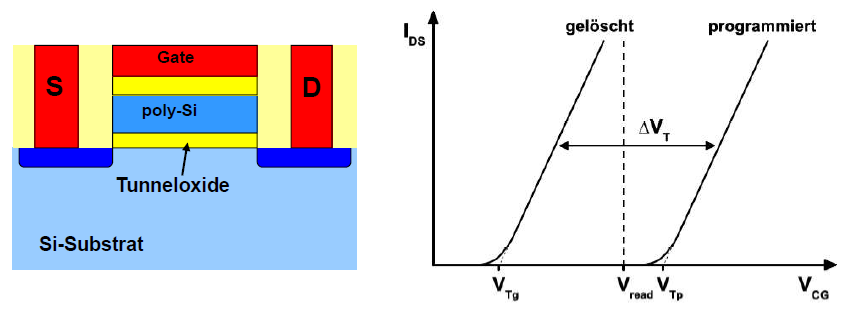
\includegraphics[width=0.5\linewidth]{Kapitel/Kap07/FloatingGate}
			\end{center}
			\item Die Anzahl der möglichen Schreibvorgänge ist auf Grund der Abnutzung (Oxiddegradationseffekten) beim Schreiben allerdings begrenzt
		\end{itemize}
	\subsubsection{Flash-EEPROM}
		\begin{itemize}
			\item portable und miniaturisierte Weiterentwicklung des EEPROMs
			\item Um die Ladungen auf das Floating Gate zu bringen wird beim Flash ein quantenphysikalischen
			Tunneleffekts (Fowler-Nordheim-Tunneln) ausgenutz, der es den Elektronen erlaubt, den Tunnelisolator zu passieren.
			\item Dies erfordert große Unterschiede im elektrischen Potential über den Isolator
		\end{itemize}
	\subsubsection{Solid State Devices}
		\begin{itemize}
			\item SSDs speichern Daten in Flash-Bausteinen
			\item Sie sind teurer aber robuster als Festplatten
			\item SSDs besitzen auf Grund möglicher Defekte des Flash Speichers in der Regel mehr Speicherzellen, um defekte Zellen zu ersetzen 
		\end{itemize}
	
	\subsubsection{Neuere Lösungen}
	\begin{itemize}
		\item Multibitspeicher (MLC)
			\begin{itemize}
				\item Es werden mehrere Bits pro Speichertransistor gespeichert
				\item Man nutzt hierzu verschiedene Ladungszustände des Transistors bzw. dessen elektrische Leitfähigkeit
			\end{itemize}
		\item Nanoclusterspeicher
		\begin{itemize}
			\item Aktuelle Floatinggates können bei einem Defekt des Tunnelisolators ihren Zustand nicht halten 
			\item Lösung: Nanocluster (Kugeln) ohne Querleitfähigkeit zwischen den einzelnen Clustern
		
			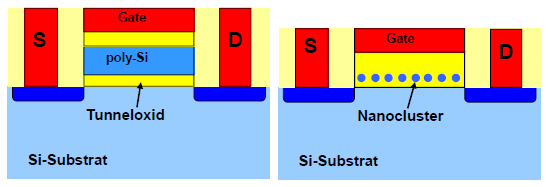
\includegraphics[width=0.3\linewidth]{Kapitel/Kap07/Nanocluster}
			
		\end{itemize}
		\item MRAM und 
			\begin{itemize}
				\item Bisherige Magnetisierung von Magnetspeichern aus der Ebene drehen
				\item ermöglicht Miniaturisieren und Skalierbarkeit
				\item Informationen werden nicht mit elektrischen sondern mit magnetischen Ladungselementen gespeichert
			
				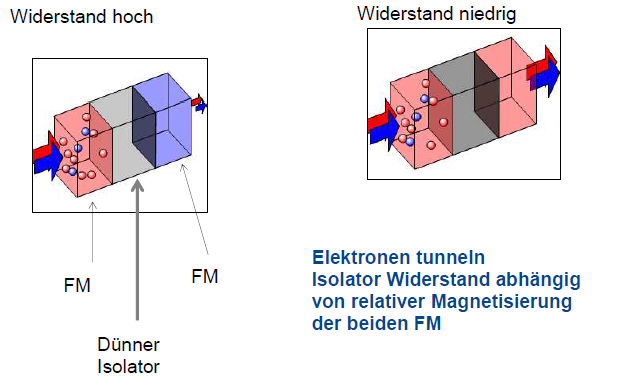
\includegraphics[width=0.3\linewidth]{Kapitel/Kap07/MRAM.png}
				
			\end{itemize}
		\item FeRAM
			\begin{itemize}
				\item Der Aufbau entspricht dem einer DRAM-Zelle. Anstelle eines konventionellen Kondensators wird ein Kondensator mit ferroelektrischem Dielektrikum eingesetzt
				
				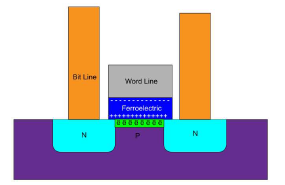
\includegraphics[width=0.2\linewidth]{Kapitel/Kap07/FeRam.png}
				
			\end{itemize}
	\end{itemize}
	

	
	





\todo{Fragen aus Own Clowd zuordnen}
\todo{Gruppenübungs-Inhalte ergänzen}